\documentclass[11pt, a4paper]{article}
\usepackage{graphicx}
\usepackage{amsmath}
\usepackage[margin=0.8in]{geometry}
\usepackage{listings}
\usepackage{float}
\usepackage{indentfirst}
\usepackage[inline]{enumitem}
\usepackage{tabularx}
\usepackage{xcolor}
\usepackage{array}
\usepackage{minted}
\usemintedstyle{vs}
\usepackage[belowskip=0pt,aboveskip=0pt,font=small,labelfont=small]{caption}
\captionsetup{width=\linewidth}
\setlength\intextsep{0pt}
\graphicspath{{Plots/}}
\setlist[itemize]{noitemsep, topsep=0pt}

\title{EE2703: Assignment 8}
\author{Sakthi Harish D T (EE19B054)}
\date{April $22^{nd}$, 2021}
\begin{document}
\maketitle
\section{Abstract:}
In this assignment, we will,
\begin{enumerate}
    \item use Symbolic Algebra in python
    \item analyse circuits using Laplace Transforms
    \item obtain response of Lowpass and Highpass Filters 
\end{enumerate}
\section{Introduction:}
In this assignment, we will analyze circuits using the Symbolic algebra  of \texttt{sympy}. Also, we will get the response of Lowpass and highpass filters for various input functions. We will use the \texttt{signal} toolbox that we used in the previous assignment.

\section{Analysis of Low-Pass Filter:}
    In this assignment, we will analyse the following Low pass Filter:
    \begin{figure}[H]
        \centering
        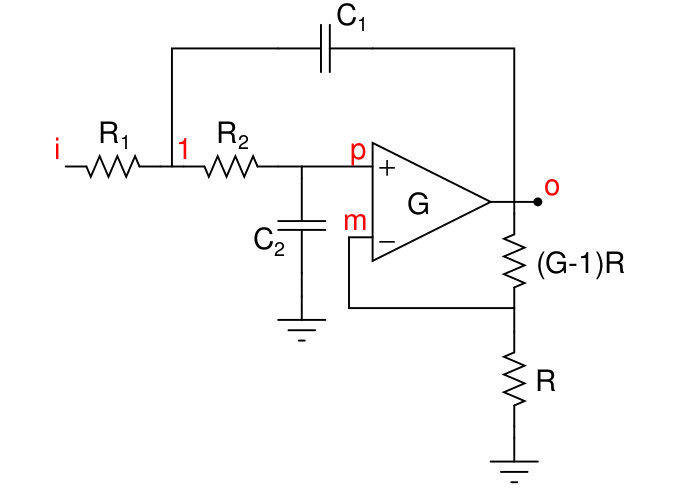
\includegraphics[scale=0.35]{lpf_ckt.png}
        \caption{Low-Pass Filter}
        \label{fig:ckt1}
    \end{figure}
    We analyse it using the Laplace transform. The values of $R_1$, $R_2$, $C_1$, $C_2$ are $10k\Omega$, $10k\Omega$, $10$pF, $10$pF respectively.\newline
    We obtain the following matrix using KCL. 
    \begin{equation}
        \begin{pmatrix}
            0&0&1&\frac{-1}{G}\\
            \frac{-1}{1+sR_2C_2}&1&0&0\\
            0&-G&G&1\\
            -\frac{1}{R_1}-\frac{1}{R_2}-sC_1&\frac{1}{R_2}&0&sC_1\\
        \end{pmatrix}
        \begin{pmatrix}
            V_1(s)\\
            V_p(s)\\
            V_m(s)\\
            V_o(s)\\
        \end{pmatrix}
        =
        \begin{pmatrix}
            0\\
            0\\
            0\\
            \frac{-V_i(s)}{R_1}\\
        \end{pmatrix}
    \end{equation}
    We solve for the voltage values and obtain the transfer function of the filter.\newline
    The obtained transfer function is a symbolic expression. But, to use
    \texttt{scipy.signal} toolbox, we need the lists containing the numerator and denominator coefficients of variable 's'. We use the following code for this conversion. 
 \textit{\textbf{Python Code:}}
    \lstset{language=Python}
    \lstset{label={lst:code_direct}}
    \lstset{basicstyle=\footnotesize}
    \begin{lstlisting}
    n,d= sp.fraction(Vo)    #this block converts Vo to list 
    n= sp.Poly(n, s)
    d= sp.Poly(d, s)
    n_coeff= n.all_coeffs() 
    d_coeff= d.all_coeffs()
    n_coeff= [float(i) for i in n_coeff]
    d_coeff= [float(i) for i in d_coeff]
    \end{lstlisting}
    Now, we can easily create a \texttt{signal.lti} object with the coefficients we got, and use \texttt{signal.step} to obtain the Step Response of the Lowpass Filter.
    \begin{figure}[H]
        \centering
        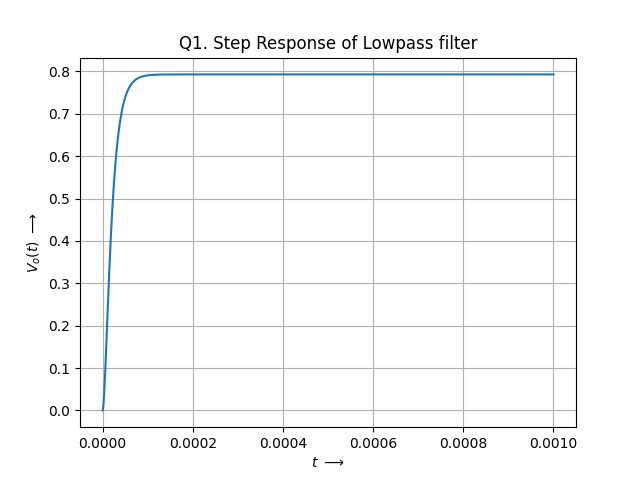
\includegraphics[scale=0.6]{Figure_1.png}
        \caption{Step response of the LPF}
        \label{fig:Fig2}
    \end{figure}
    Now, we give an input which has both Low and High frequency components. Since it is a Lowpass filter, the output voltage should contain only the low frequency component.

    \begin{equation}
        v_i(t) = (sin(2\pi\times 10^3t)+cos(2\pi\times 10^6t))u(t)
        \label{eq4}
    \end{equation}
    
    We shall use \texttt{signal.lsim} to obtain the output voltage of the circuit.
    \begin{figure}[H]
        \centering
        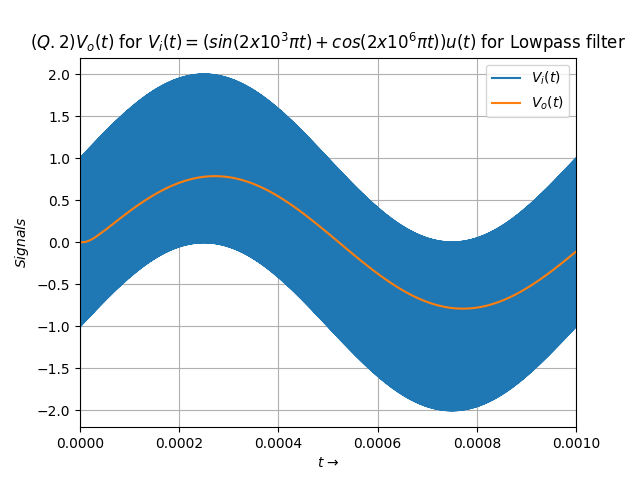
\includegraphics[scale=0.6]{Figure_2.png}
        \caption{$v_o(t)$ for the given $v_i(t)$}
        \label{fig:Fig2}
    \end{figure}
    
    We can easily see that the output contains only the low frequency component of the input ($1\ KHz$ sinusoid). Thus, the circuit is a low-pass filter. 
\section{Analysis of High-Pass Filter:}

Now, we analyse a Highpass filter with the values of components as $R_1$, $R_2$, $C_1$, $C_2$ are $10k\Omega$, $10k\Omega$, $1$nF, $1$nF, respectively.
\begin{figure}[H]
    \centering
    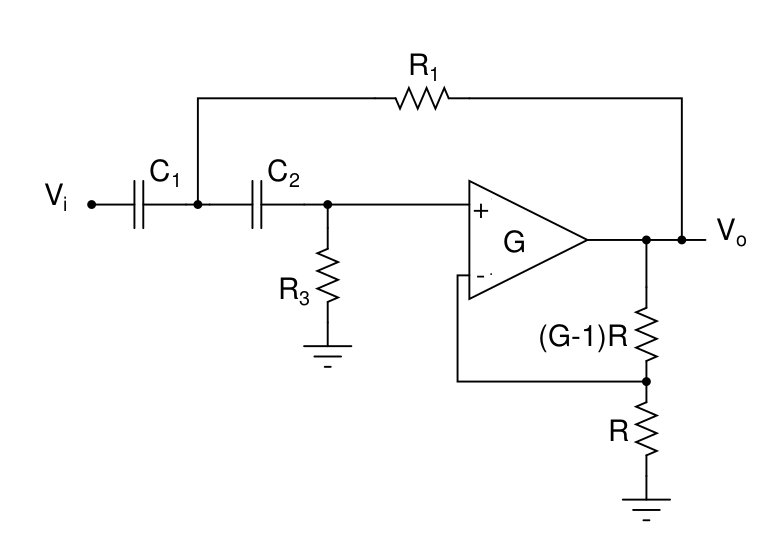
\includegraphics[scale=0.35]{hpf_ckt.png}
    \caption{High-Pass Filter}
    \label{fig:fig5}
\end{figure}

Performing a similar procedure like before, we get the KCL matrix as:
\begin{gather}
    \begin{pmatrix}
            0&0&1&\frac{-1}{G}\\
            \frac{sR_3C_2}{1+sR_3C_2}&0&-1&0\\
            0&-G&G&1\\
            -\frac{1}{R_1}-sC_2-sC_1&0&sC_2&\frac{1}{R_1}\\
        \end{pmatrix}
        \begin{pmatrix}
            V_1(s)\\
            V_p(s)\\
            V_m(s)\\
            V_o(s)\\
        \end{pmatrix}
        =
        \begin{pmatrix}
            0\\
            0\\
            0\\
            -sC_1V_i(s)\\
        \end{pmatrix}
\end{gather}
We use \texttt{sympy.lambdify} to use the symbolic expression in supported format to plot the Magnitude response of the Highpass filter. 
\begin{figure}[H]
    \centering
    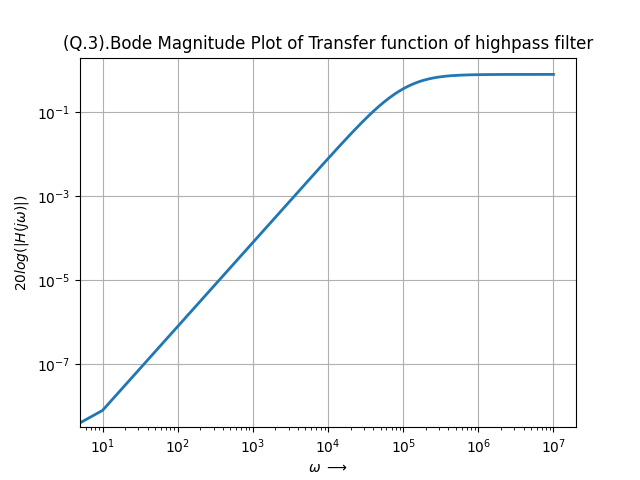
\includegraphics[scale=0.6]{Figure_3.png}
    \caption{Magnitude response of HPF}
    \label{fig:Fig6}
\end{figure}
We now give the mixed frequency input to the HPF. \newline
The response to the mixed frequency input in Eq \eqref{eq4} is:
\clearpage
    \begin{figure}[H]
        \centering
        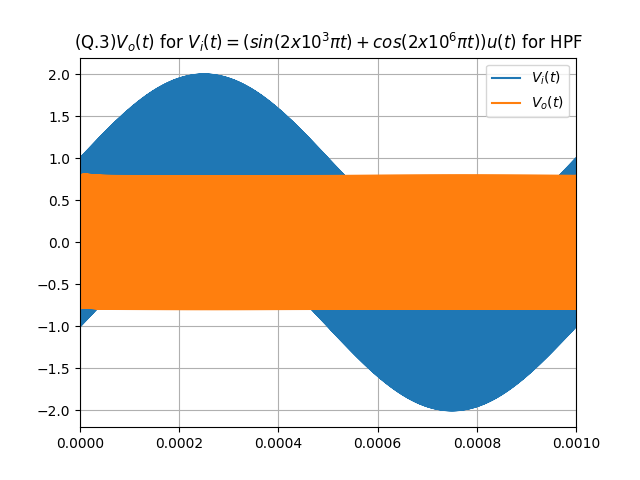
\includegraphics[scale=0.6]{Figure_4.png}
        \caption{$v_o(t)$ for the given $v_i(t)$}
        \label{fig:Fig2}
    \end{figure}
We can see that the output contains only the high frequency component of the input, which is expected because the system is a Highpass filter.
    \newline\newline\newline
Next, we shall look at the response of the system to a damped sinusoid. We shall consider two of them - one of low frequency (0.5 kHz) and the other of high frequency (0.5 MHz).

\begin{figure}[H]
    \centering
    \setlength\tabcolsep{1pt}
    \begin{tabular}{cc}
        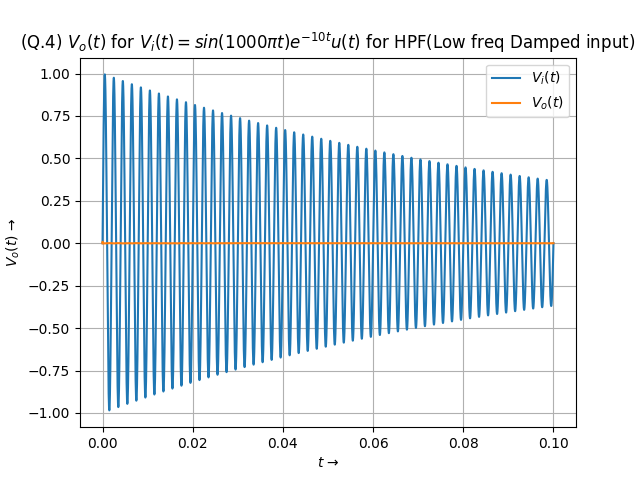
\includegraphics[width=0.55\textwidth]{Figure_5.png} &
        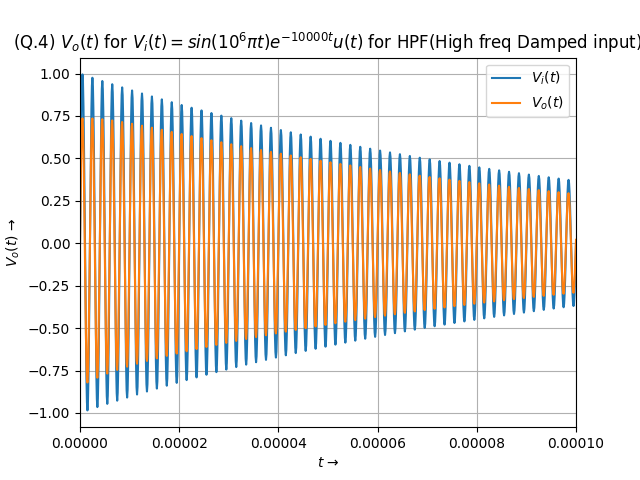
\includegraphics[width=0.55\textwidth]{Figure_6.png}\\
    \end{tabular}
    \caption{\textit{Left}: Low frequency input\\\textit{Right}:High frequency input}
\end{figure}

We get that the output of the filter is 0, if the input is a low frequency damped sinusoid. This is as expected due to the inherent nature of the circuit to act as a high-pass filter. This is why we can see that it allows the high-frequency input to pass through.
\newline\newline\newline
We now give a Unit step function as the input and obtain the step response of the system.
The step response of the circuit was obtained as:

\begin{figure}[H]
    \centering
    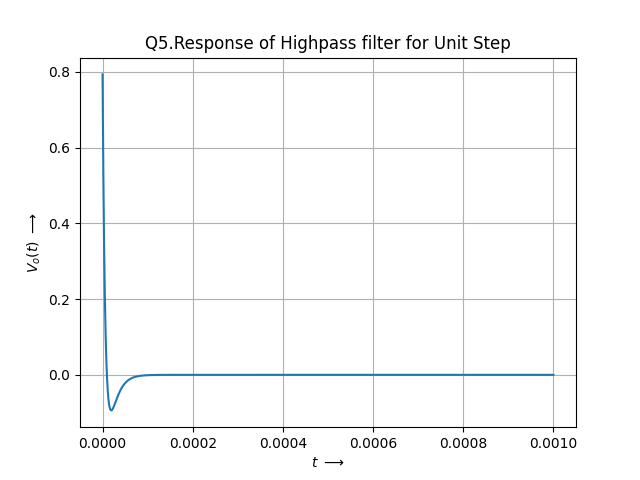
\includegraphics[scale=0.6]{Figure_7.png}
    \caption{Step Response of HPF}
    \label{fig:Fig7}
\end{figure}
As expected , the Step response of the Highpass Filter is zero because the filter doesn't allow DC signal to pass through. The under-shoot in the beginning is due to initial transients which die out as time passes. 


\section{Conclusion}
\begin{enumerate}
    \item \texttt{Sympy} provides a useful way to analyse LTI systems using the Laplace transforms. 
    \item  We studied the behaviour of a low pass filter,realized using an operational amplifier of gain G.
    \item   For a mixed frequency sinusoid as input,  it  was  found  that  the  filter  suppressed  the  high  frequencies  while allowing  the  low  frequency  components. 
    \item     Similarly,  a  high  pass  filter  was implemented using an operational amplifier with the same gain.  The magnitude response of the filter was plotted and its output was analysed for damped sinusoids.
    \item The step response of the filter was found to have a non-zero peak at $t= 0$ ,due to the sudden change in the input voltage(initial transients).


\end{enumerate}
\end{document}
